%%% File encoding: UTF-8
%%% äöüÄÖÜß  <-- no German umlauts here? Use an UTF-8 compatible editor!

%%% Magic comments for setting the correct parameters in compatible IDEs
% !TeX encoding = utf8
% !TeX program = pdflatex 
% !TeX spellcheck = de_DE
% !BIB program = biber

\RequirePackage[utf8]{inputenc} % Remove when using lualatex or xelatex!
\RequirePackage{hgbpdfa}        % Creates a PDF/A-2b compliant document



\documentclass[bachelor,english,smartquotes]{hgbthesis}
% Valid options in [..]: 
%    Type of work: 'diploma', 'master' (default), 'bachelor', 'internship' 
%		 Additionally for a thesis exposé: 'proposal (for 'bachelor' and 'master')
%    Main language: 'german' (default), 'english'
%    Turn on smart quote handling: 'smartquotes'
%    APA bibliography style: 'apa'
%%%-----------------------------------------------------------------------------
\usepackage{tikzpeople}

\usepackage{siunitx}
\sisetup{per-mode=symbol}
%\sisetup{quotient-mode=fraction} % Output a/b as \frac{a}{b}

\usetikzlibrary{positioning,fit,arrows.meta,backgrounds}

\tikzset{
    module/.style={%
        draw, rounded corners,
        minimum width=#1,
        minimum height=7mm,
        font=\sffamily
    },
    module/.default=2cm,
    >=LaTeX
}

\tikzstyle{arrowUni} = [draw, ->]
\tikzstyle{arrowBi} = [draw, <->]

\lstnewenvironment{myverbatim}[1][]{%
    \lstset{
        basicstyle=\ttfamily,
        frame=tb,
        #1
    }%
}{}


\newlist{encase}{enumerate}{1}
\setlist[encase]{label=Case \arabic*:, leftmargin=2cm}


\graphicspath{{images/}}  % Location of images and graphics
\logofile{logo}           % Logo file: images/logo.pdf (no logo: \logofile{})
\bibliography{BA_Scheuchenpflug} % Biblatex bibliography file (references.bib)


%%%-----------------------------------------------------------------------------
\begin{document}
%%%-----------------------------------------------------------------------------

%%%-----------------------------------------------------------------------------
% Title page entries
%%%-----------------------------------------------------------------------------

\title{Integration of Driving- and Trafficsimulation}
\author{Martin Scheuchenpflug}
\programname{Universal Computing}

%\programtype{Fachhochschul-Bachelorstudiengang} % select/edit
\programtype{Automotive computing}

\placeofstudy{Hagenberg}
\dateofsubmission{2024}{06}{25} % {YYYY}{MM}{DD}

\advisor{FH-Prof. Dr. Gerald Ostermayer} % optional

%\strictlicense % restrictive license instead of Creative Commons (discouraged!)

%%%-----------------------------------------------------------------------------
\frontmatter                                   % Front part (roman page numbers)
%%%-----------------------------------------------------------------------------

\maketitle
\tableofcontents

\include{front/preface} % A preface is optional
\include{front/abstract}		
\include{front/kurzfassung}			

%%%-----------------------------------------------------------------------------
\mainmatter                                    % Main part (arabic page numbers)
%%%-----------------------------------------------------------------------------
\chapter{Introduction}\label{ch:introduction}

\section{Motivation}\label{sec:motivation}
    \subsection{Driving simulation}\label{subsec:driving-simulation}
        The use of driving simulators is common practice among researchers for studying driving behaviors in scenarios that may include dangerous and unlikely situations\cite{Wynne2019,That2011}.
        % TODO: reformulate
        Utilization of driving simulators is primarily driven by the significant reduction in time and financial resources for engineers and developers, as evidenced by reference\cite{That2011}.
        Additionally, it facilitates expeditious research and evaluation of innovative human-machine-interface designs (HMI) within the automotive industry\cite{riegler2023}.
        % "me"-perspective zittieren?
        One such simulator represents the "me"-perspective by focusing the simulation on the vehicle that is driven by a human in the simulator, thereby ensuring that this vehicle is modeled with great precision.
        One illustrative example of a well-known driving simulator is CARLA, which is an open-source, free-to-use driving simulator with a feature-rich Python API\cite{carla2017}.

    \subsection{Microscopic traffic simulation}\label{subsec:microscopic-traffic-simulation}
        The use of microscopic traffic simulators is also a common methodology among researchers studying the dynamics of vehicular traffic, particularly in the context of intelligent transportation systems (ITS)\cite{toledo2005microscopic}.
        One such microscopic traffic simulator employs (among other models like: lane-change, fuel-consumption, \ldots) car-following models to regulate the acceleration and, consequently, the movement of each vehicle\cite{treiber2013traffic}.
        A variety of car-following models are available to use for modelling different types of vehicles.
        One notable example is the IDM (Intelligent Driver Model) (see Section~\ref{subsec:intelligent-driver-model}) described by Springer et al., which assembles a complete and accident free models, that produces plausible acceleration profiles\cite{treiber2013traffic}.
        % TODO:Richtig Zittiert??
        Moreover, as described in~\cite{treiber2013traffic} these models are derived from a set of assumptions about real drivers such as keeping a "safe distance" from the leading vehicle, driving at a desired speed or preferring acceleration to be within a comfortable range, etc.
        As all the mentioned Parameters are like sensor-values to a modern ACC (adaptive cruse control) System with the model being the control system.
        Since these models are fully deterministic, they don`t model the "errors" of human drivers.

    \subsection{Integrated simulation environment}\label{subsec:integrated-simulation-environment}

        \begin{figure}
            \centering
            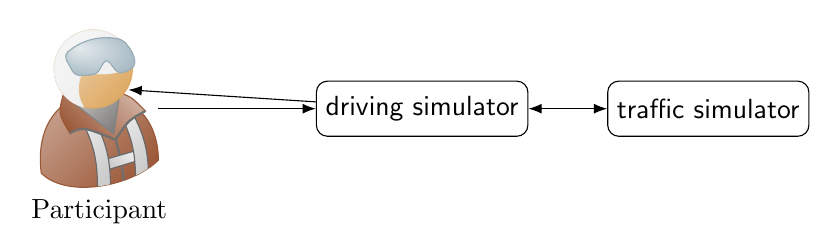
\begin{tikzpicture}[scale=5]
                \node[name=p, shape=pilot, minimum size=1.5cm](P1){Participant};
                \node[module, right= 2cm of P1] (I1) {driving simulator};
                \node[module, right= 1cm of I1] (I2) {traffic simulator};
                \draw[<->] (I1)--(I2);
                \draw[->] (I1)--(P1.mouth);
                \draw[->, ] (P1.east)--(I1);
            \end{tikzpicture}
            \caption{Integration architecture}
            \label{fig:int:architecture}
        \end{figure}

        The goal of investigating the impact of human drivers on traffic flow can be achieved by modeling those imperfections of a human driver.
        Using so called meta-models on top of  typical vehicle-following models which modify the behavior to closely match a real human driver.
        Example for meta-models are the human driver model (HDC)\cite{treiber2006delays} or the extended human driver model (EHDC)\cite{Lindorfer2018}.
        An additional potential methodology for the observation of human behavior is to engage directly in a scenario, which offers the benefit of eliminating the necessity for a model of the human driver.
        As a result of the direct participation of the human in the scenario, the impact of that behavior on the overall traffic flow can be observed.
        The aforementioned "me"-perspective is transformed into a holistic "we"-perspective through the utilization of an integrated simulation environment~\cite{riegler2023}.
        This kind of integration has proven very useful\cite{punzo2010integration}.

        There are two types of integrations:
        \begin{itemize}
            \item \textbf{Offline integration:} For this integration a driving simulator and a traffic simulator are used seperatly.
            For example one could build the same scenario in both simulators and a human driver could participate in the scenario inside the driving simulator.
            Afterward the behavior of the human driver is recorded and imported into the traffic simulator, so the impact of the recorded behavior can be observed.
            The key disadvantages of this integration are, that it lacks the possibility of observing the impact of the driving behavior in real time and the model-controlled vehicles are not able to adapt to the human driver's behavior during the simulation.
            \item \textbf{Online integration:} The aforementioned disadvantages are rendered obsolete by implementation of an online integration.
            The most straightforward structure for such an integration would be to have the participant interact with the driving simulator, which is then synchronized to the traffic simulator.
            This can be achieved by connecting a driving simulator with a microscopic traffic simulator, as illustrated in Figure\ref{fig:int:architecture}.
            By running the simulators in sync, it is possible for the simulation controlled (by the traffic simulator) vehicles to react to the driving actions of the vehicle controlled by a human driver.
        \end{itemize}
        The remaining work focuses on the online integration of the simulators, unless otherwise specified.

\section{Objective of the work}\label{sec:objective-of-the-work}
    In this thesis, an integrated Simulation Environment is proposed, consisting of the driving simulator CARLA\cite{carla2017} and the microscopic traffic simulator TraffSim\cite{backfrieder2013traffsim,backfrieder2014traffsim}.
    The primary objective of this integration is to achieve a robust and synchronized environment, where the real-time interactions between human-driven and vehicular-follow-model-controlled vehicles unfold seamlessly.

    The key challenges of the proposed integrated environment are:
    \begin{itemize}
        \item \textbf{Synchronisation of integration components:} {
            One of the primary objectives of this work is to ensure seamless synchronisation between the driving and traffic simulators.
            This synchronisation involves real-time data exchange, particularly for online integration, where the actions of a human driver in the driving simulator should immediately impact vehicle behaviours in the traffic simulator.
            A significant challenge in this regard is the minimisation of latency, which could cause inconsistent or delayed responses between simulators.
        }
        \item \textbf{Road network compatibility and flexibility:}{
            Synchronizing road networks across the simulators is essential for a coherent simulation environment, as inconsistencies can lead to inaccuracies in traffic flow or navigation.
            Therefore, a procedure for exporting, importing and exchaning road networks between the simulators was implemented by the use of the OpenDrive\ref{openDrive} Standard.
        }
        \item \textbf{Handling human driving behavior:}{
            Human drivers often exhibit unpredictable behaviors, creating a need for adaptable models that can respond effectively to erratic or non-standard actions.
            This objective was partially archived by extrapolating the acceleration and speed of human-driven vehicle, for further use, this objective has to be readressed.
            One potential solution for this problem could be to use a vehicle-following, which models a human driver\cite{Lindorfer2018}, to predict the next action taken by the human in charge of the vehicle.
        }
    \end{itemize}

\section{Structure}\label{sec:structure}
    This thesis is structured into multiple chapters, each addressing discrete aspects of the integration of driving and traffic simulators and the associated challenges.\\

    The initial chapter, entitled "Introduction", provides an overview of the subject, outlining the historical development of driving and traffic simulation, the individual functionalities of each, and the rationale for integrating them into a unified environment.
    Furthermore, it delineates the objectives and scope of the work.

    The second chapter, entitled "Basics", identifies the foundational studies of the field of traffic research, that are related to the discussed topic.

    The third chapter, entitled "Related Work", presents a review of existing research on driving and traffic simulation systems.
    It focuses on previously explored methods for integration, identifying both successful techniques and common obstacles encountered.

    The fourth chapter, entitled "Methods", provides a detailed account of the architectural design of the integrated simulation environment.
    It describes the technical framework and design decisions that have been taken in order to achieve synchronisation of the simulators, to facilitate real-time data exchange and to ensure compatibility between simulator platforms.

    The fifth chapter, Results, presents the outcomes of the implemented integration, including a discussion of performance metrics, an analysis of the observed behaviours of the simulation components, and an evaluation of the solutions proposed for specific integration challenges.

    The sixth chapter, entitled "Future Work", identifies areas for further research and development.
    It mainly discusses future use cases for the proposed integrated environment in addition to a description of the necessary steps to transform the already working proof of concept into a usable tool for traffic research.
\chapter{Related work}\label{ch:related-work}
    In the following chapter provides an overview of research and state-of-the-art in the domain of modelling and simulation of traffic systems.
    Section~\ref{sec:foundational-studies} examines foundational studies that have shaped current understanding of modelling traffic systems, focusing on the methodologies and findings that are most relevant to this thesis.
    Section~\ref{sec:studies-closely-related-to-an-integrated-simulation-environment} focuses on studies that are more closely related to the proposed simulation environment and the challenges that had to be solved in order to create one such integration.
    Finally, Section~\ref{sec:summary-of-findings} summarises the findings of the literature review and identifies the used solutions for upcoming challenges encountered along the way of developing the integrated Simulation environment.
    By mapping out the state of the art, this chapter establishes the context for the subsequent discussion of the proposed approach and methodology in Chapter~\ref{ch:methods}.


    \section{Foundational studies}\label{sec:foundational-studies}
        The field of traffic science is divisible into multiple different sub-categories by the time span of the observed events.
        As described by Treiber et al. \cite{treiber2013traffic} there are Vehicle dynamics, Traffic flow dynamics and Transportation planning as the three major topics(see Table~\ref{tab:dilimination-of-traffic-flow-dynamics}).
        These fields are divisible even further as stated in table~\ref{tab:dilimination-of-traffic-flow-dynamics}.
        The proposed simulation environment would fall into the category of traffic flow dynamics using microscopic car following models.
        According to Treiber et al. this kind of simulation environments are best used to model reaction times, time gaps and the acceleration/breaking behaviors of vehicles in a traffic scenario.
        Driving behavior of vehicles in traffic flow dynamics are usually described by vehicle following (VF) models, which will be discussed further in the following sections.

        \begin{table}[ht]
            \centering
            \begin{tabular}{p{.1\linewidth} p{.2\linewidth} p{.2\linewidth} p{.4\linewidth}}
                \hline
                Time scale & Field & Models & Aspects of traffic (examples) \\ \hline \hline
                $\le 0.1 s$ & Vehicle dynamics & Sub-microscopic & Control of engine and breaks \\ \hline
                1 s & \multirow{4}{\linewidth}{Traffic flow dynamics}&\multirow{2}{\linewidth}{Car-following modells} & Reaction time, time gap \\
                10 s & & & Acceleration and deceleration \\\\
                1 min& & \multirow{2}{\linewidth}{Macroscopic models} & Cycle period of traffic lights \\
                10 min & & & Stop-and-go waves \\ \hline
                1 h & \multirow{5}{\linewidth}{Transportation planning} & \multirow{3}{\linewidth}{Route assignment traffic demand} & Peak hour \\
                1 day & & & Daily demand pattern \\
                1 year & & & Building/changing infrastructure \\\\
                5 years & &  \multirow{2}{\linewidth}{Statistics age pyramid} & Socioeconomic structure \\
                50 years & & & Demographic change \\ \hline

            \end{tabular}
            \caption{Delimitation of traffic flow dynamics from vehicular dynamics and transportation planning\cite{treiber2013traffic}}
            \label{tab:dilimination-of-traffic-flow-dynamics}
        \end{table}

        \subsection{Gazis-Herman-Rothery model}\label{subsec:gazis-herman-rothery-model}
            Vehicle following models have been researched for more than 70 years~\cite{pipes1953operational} and many such models have been developed since.
            One of the first widely known VF models is the Gazis-Herman-Rothery (GHR) model (see Eq \ref{eq:GHR}), which described the acceleration of a vehicle $n$ in a driving scenario with respect to the difference in speed $\Delta v$ to the leading vehicle $n-1$ and the distance to the leading vehicle $\Delta x$, at a point earlier in time, with $T$ being the reaction time of the driver\cite{Brackstone1999}.
            \begin{equation}
                a_n(t) = c v_n^m(t) \frac{\Delta v (t-T)}{\Delta x^{-1} (t-T)} \label{eq:GHR}
            \end{equation}

        \subsection{Gipps' model}\label{subsec:gipps-model}
            Gipps states in the paper proposing his own VF model (Gipps´ model), that most VF models up until then (1981) have generally been in the form of EQ~\ref{eq:general-form-vf-model-1981}, where $\tau = T$.
            One example for this general form is the GHR model, some more of those models are found in publications dating back to that time: \cite{newell1961nonlinear, lee1966generalization, bender1970flow}.
            \begin{equation}
                a_n(t+\tau) = l_n \frac{[v_{n-1} - v_n]^k}{[x_{n-1} - x_n]^m}\label{eq:general-form-vf-model-1981}
            \end{equation}
            As pointed out by Philip A. Seddon, the fact, that the time interval between subsequent calculations was given by the reaction time was an undesired characteristic of these models\cite{seddon1972program}, which could be overcome by storing a considerable amount of historical data, which was undesired at the time.
            The second pain point of these models, by today's standards maybe the more relevant point, was the existence of parameters $l_n$,$k$,$m$ (EQ~\ref{eq:general-form-vf-model-1981}), that have no identifiable connection to driver or vehicle characteristics\cite{gipps1981behavioural}.

            To address these deficits, Gipps proposed a new vehicle following model describing the speed of a vehicle at a point in time, in contrast to describing the acceleration of a vehicle at a point in time.
            The following form of the Gipps` model is not the form of the original publication, but the form from~\cite{treiber2013traffic}, which introduces a save speed $v_{save}$ for simplification.
            As stated by Treiber et al. the model is conseptually unchanged.
            The GHR model calculates the speed of a vehicle with respect to the desired acceleration $a$, deceleration $b$, Desired speed $v_0$ and minimum distance $s_0$.
            \begin{align}
                v_{save} (s, v_l) &= -b*\Delta t + \sqrt{b^2 \Delta t^2 - v_l^2 + 2b (s-s_0)} \\
                v(t+ \Delta t) &= min[v+a\Delta t, v_0, v_{save}(s,v_l)] \label{eq:gipps-model-simplified}
            \end{align}
            With the concept of the save speed depending on the distance to the front vehicle $s$ and its speed $v_l$, the gipps` model assembles one of the simplest complete %TODO: explain model completeness
            and accident-free models possible.
            The accident-free characteristic of the model is guaranteed with the assumptions that deceleration and reaction times are constant~\cite{treiber2013traffic}.
            In essence the gipps` model chooses the minimum between the desired speed, the safe speed or the speed that max acceleration would result in the next time step.
            Problem with this model is, that as stated by Treiber et al. it produces an unrealistic acceleration profile.

        \subsection{Intelligent driver model}\label{subsec:intelligent-driver-model}
            The time-continuous Intelligent driver model produces a realistic acceleration profile, since one of the requirements for forming the IDM is that the acceleration function $\dot{v}(s,v,v_l)$ is continuously differentiable in every three variables and thus producing smooth transitions between eg. breaking and acceleration phases.
            Another design criteria of the IDM is that the equilibrium distance\footnotemark has to be larger than the "safe" distance ($v*T + v_0$), with $v$ being the current speed, $T$ being the desired distance between vehicles in seconds and $v_0$ representing the "bumper-to-bumper" distance (min distance kept between vehicles), which ensures the accident-free characteristic of that model.
            \footnotetext{The Distance, that is required between vehicles to stay in a steady-state equilibrium, which means, in a homogenous convoy the distance between all vehicles and the speed is the same. Furthermore the acceleration has to be 0 for every vehicle to be in a steady-state eqilibrium. \cite{treiber2013traffic, treiber2000IDM} }

            \begin{align}
                s^*(v,\Delta v) = s_0 + \max\left( 0, vT + \frac{v \Delta v}{2 \sqrt{ab}} \right) \label{eq:IDM-s-star} \\
                \dot{v}(s,v,v_l) = a * \left[ 1- \left(\frac{v}{v_0}\right)^\delta  - \left( \frac{s^*(v, \Delta v)}{s} \right)^2\right] \label{eq:IDM}
            \end{align}

            The IDM (see EQ~\ref{eq:IDM})is constructed from 2 pieces, the first part is comparing the current speed to the desired speed: $\left(\frac{v}{v_0}\right)^\delta$.
            The second part is comparing the current distance to the desired distance $s^*$ (see EQ~\ref{eq:IDM-s-star}): $\left( \frac{s^*(v, \Delta v)}{s} \right)^2$ \cite{treiber2013traffic, treiber2000IDM}.

            The advantage of using an intuitive model like gipps` model or the IDM, is that they are easy to configure by some simple understandable parameters (including vehicle and driver specific numbers).
            For example the configuration of the IDM consists of six parameters controlling the behavior of vehicles, with default values used by TraffSim (see Table~\ref{tab:IDM-Default-Values})~\cite{treiber2013traffic,backfrieder2013traffsim,backfrieder2014traffsim}.
            The Implementation in TraffSim includes two additional parameters, determining the maximum possible acceleration $a_{max}$ and deceleration $b_{max}$, which act as a hard limit for the acceleration function.
            The value of $b_{max}$ for example models the physical limit of the breaks of a car.
            \begin{table}
                \centering
                \begin{tabular}{l c c}
                    Parameter & TraffSim default Value & Acceptable Range \\
                    \hline
                    Comfortable acceleration $a$ & $2 \si{\m\per\s\squared}$ & $ 0 < a < a_{max}$\\
                    Comfortable deceleration $b$ & $-2 \si{\m\per\s\squared}$ & $ b_{max} < b < 0$\\
                    Desired Speed $v_0$ & $25 \si{\m\per\s}$ & $v_0 > 0$ \\
                    Minimum bumper-to-bumper distance $s_0$ & $2 \si{\m}$ & $s_0 > 0$ \\
                    Time gap $T$ & $1.5 \si{\s}$ & $T > 0$\\
                    Acceleration exponent $\delta$ \footnotemark& 4 & $\delta >  0$\\
                \end{tabular}
                \caption{Default Values for IDM}
                \label{tab:IDM-Default-Values}
            \end{table}
            \footnotetext{Dimensionless factor determining the rate at wich the vehicle`s acceleration decreases as it approaches its desired velocity}

        \subsection{Micro traffic simulation}\label{subsec:micro-traffic-simulation}
            The aforementioned vehicle following models are among others, implemented in a traffic simulator.
            Since one such simulator is a key building block of the desired simulation environment, the next section focuses on the micro traffic simulation environments available in literature.
            Special focus will be placed onto the micro traffic simulator TraffSim~\cite{backfrieder2013traffsim,backfrieder2014traffsim}, developed in house at Hagenberg.

            The first notable example is MovSim~\cite{Treiber2010}, which is an open source, free to use traffic simulator developed by a team at TU Dresden.
            MovSim implements the IDM (see Section~\ref{subsec:intelligent-driver-model}) among other vehicle following model which is responsable for the longitudinal movement of vehicles.
            For transversal movement of vehicles, MovSim utilizes the MOBIL model~\cite{kesting2007general}, which is a model for lane changing working alongside a variety of VF models.
            MovSim is primary source for sample implementations of VF models described by Treiber et al. (in~\cite{treiber2013traffic}).
            A picture of the web based user interface is depicted in Figure~\ref{fig:mov-sim-ui}.

            \begin{figure}
                \centering
                \includegraphics[width=0.7\textwidth]{Movsim}
                \caption{MovSim user interface~\cite{MovSimUI}}
                \label{fig:mov-sim-ui}
            \end{figure}

            One of the most popular traffic simulation environments is Eclipse SUMO~\cite{Behrisch2011SUMOS}, which is


    \section{Studies closely related to an integrated simulation environment}\label{sec:studies-closely-related-to-an-integrated-simulation-environment}

    \section{Summary of findings}\label{sec:summary-of-findings}

    As described by Treiber et al., both of these simulators are located in the field of traffic flow dynamics.



    \section{Microscopic traffic simulation}\label{sec:microscopic-traffic-simulation}


    \section{Driving simulation}\label{sec:driving-simulation}



\chapter{Methods}\label{ch:methods}

\section{Architecture of the Integrated Simulation Environment}\label{sec:architecture-of-the-integrated-simulation-environment}
    The proposed integration consists of the open-source Driving Simulator CARLA\cite{carla2017} and the microscopic traffic simulator TraffSim\cite{backfrieder2013traffsim,backfrieder2014traffsim}, which was developed at the University of Applied Sciences Upper Austria.
    To connect the two simulators into one integrated environment, a gRPC\cite{wang1993grpc} API was added to the microscopic traffic simulator, as well as a REST (Representational State Transfer) Endpoin.
    The gRPC-API is used to transfer data between the simulators during a running Simulation, as well as to transfer control signal (such as: Pausing the Simulation).
    The REST-Endpoint is used by the driving simulator to request the map used for the scenario.
    This map is requested in OpenDrive Format (see Section\ref{sec:road-network-export-and-sync}).

    \subsection{Vehicles in TraffSim}\label{subsec:vehicles-in-traffsim}
        In TraffSim there are a few different Types of Vehicles (see Figure %TODO )

\subsection{Simulation step synchronisation}\label{subsec:simulation-step-synchronisation}
        \begin{figure}
            \centering
            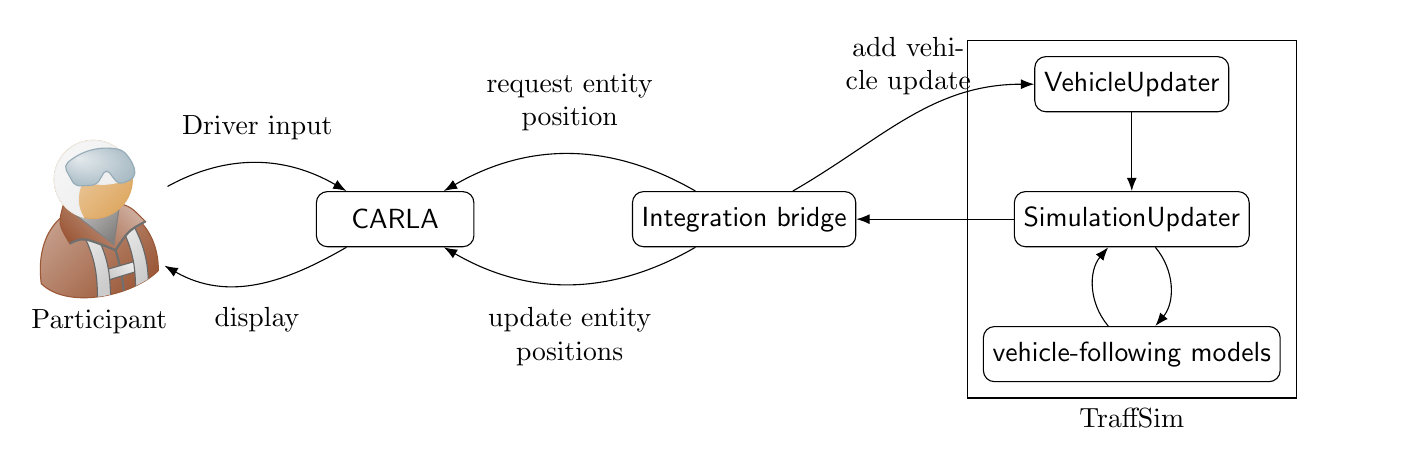
\begin{tikzpicture}
                \node[name=p, shape=pilot, minimum size=1.5cm](uInput){Participant};
                \node[module, right= 2cm of uInput](dSim){CARLA};
                \node[module, right= 2cm of dSim](bridge){Integration bridge};
                \node[module, right= 2cm of bridge](su){SimulationUpdater};
                \node[module, above= 1cm of su](hdvu){VehicleUpdater};
                \node[module, below= 1cm of su](vfm){vehicle-following models};
                \node[fit=(su) (hdvu) (vfm), draw, inner sep=2mm] (tSim){};
                \node[below] at (tSim.south){TraffSim};

                \path[arrowUni] (uInput) to[out=30, in=150] node [text width=2.5cm,midway, above=0.5em,align=center ] {Driver input} (dSim);
                \path [arrowUni] (bridge) to[out=150, in=30] node [text width=2.5cm,midway, above=0.5em,align=center ] {request entity position} (dSim);
                \path [arrowUni] (bridge) to[out=30, in=180] node [text width=2.5cm,midway, above=0.5em,align=center ] {add vehicle update} (hdvu);
                \path [arrowUni] (hdvu) -- node [text width=2.5cm,midway, right=0.5em,align=center ] {} (su);
                \path [arrowUni] (su) to[out=-50, in=50] node [text width=2.5cm,midway, right=0.5em,align=center ] {} (vfm);
                \path [arrowUni] (vfm) to[out=130, in=-130] node [text width=2.5cm,midway, left=0.5em,align=center ] {} (su);
                \path [arrowUni] (su) -- node [text width=2.5cm,midway, left=0.5em,align=center ] {} (bridge);
                \path [arrowUni] (bridge) to[out=-150, in=-30] node [text width=2.5cm,midway, below=0.5em,align=center ] {update entity positions} (dSim);
                \path [arrowUni] (dSim) to[out=-150, in=-30] node [text width=2.5cm,midway, below=0.5em,align=center ] {display} (uInput);
            \end{tikzpicture}
            \caption{Data roundtrip}
            \label{fig:architecture-integration}
        \end{figure}
        The human driver employs the Carla interface to engage with the integrated simulation environment (see Figure\ref{fig:architecture-integration}).
        It is essential that the driving behaviour of the simulation-controlled vehicle appears natural to the human driver.
        Therefore, the time between driver input and the visual output of the driving simulator must be minimised (data round-trip time).
        It is essential that the driver's input is accurately captured by Carla and that the human-driven vehicle is precisely simulated in order to create a realistic driving experience for the driver.
        As the two simulators are not synchronised with regard to their tick rates, the integration bridge requests the current position, speed and acceleration of the vehicle and a vehicle update is added to the update queue of the HumanDrivenVehicleUpdater within the traffic simulator.
        Upon calculation of the subsequent simulation step in the traffic simulator, all vehicle updates that have been queued are executed, thereby updating the human-driven vehicle.
        Therefore, the delta time between simulation steps should be selected as low as possible, in order to minimise the data round-trip time.


    \subsection{Real time simulation}\label{subsec:real-time-simulation}
        %FIXME: redo
        although $t$ must not be lower than the time it takes for the simulation step to be calculated $T$.
        To bind the simulation time to the real time, the easiest way would be to set the time step size to the time duration it took for the last simulation step to compute:
        \[
            t_{x} = T_{x-1}
        \]
        The problem with that approach is, that during a simulation in TraffSim it should be avoided to change the simulation step $t$, so another approach is used, by adding a delay after each simulation step to compensate for the difference between $t$ and $T$.
        It`s important for this technique to work, the condition $t \geq T$ has to be met.
        In every simulation step the added delay $d$ has to be calculated and thus $t$ can be static:
        \[
            d_{x} = t - T_x
        \]

\section{TraffSim API}\label{sec:traffsim-api}
    To interact with the microscopic traffic simulator TraffSim, a gRpc\cite{wang1993grpc} API was specified and developed, which allows the client to call the functions described in Listing\ref{lst:traffSim-api-proto}.
    The Api was designed to allow the client to control all the functions that are important during a simulation session and also to sync the two simulators.



\begin{GenericCode}[caption={TraffSim API proto}, label={lst:traffSim-api-proto}]
service TraffSimController {
    rpc requestVehicleData (ActiveSimulationRun)
        returns (VehicleData);
    rpc notifyFreeDrivingVehicle(FreeDrivingVehicleUpdateRequest)
        returns(VoidMessage){}
    rpc simulationAllowTswConnection (ActiveSimulationRun)
        returns (BoolMessage) {}
    rpc getAvailableFreeDrivingVehicles(ActiveSimulationRun)
        returns(AvailableFreeDrivingVehicles){}
    rpc getAvailableScenarios (VoidMessage)
        returns (AvailableScenarios){}
    rpc getOpenSimulations (VoidMessage)
        returns (ActiveSimulationRuns){}
    rpc getSimulationState (ActiveSimulationRun)
        returns (SimulationState){}
    rpc pauseSimulation (ActiveSimulationRun)
        returns (VoidMessage){}
    rpc startSimulation (ActiveSimulationRun)
        returns (VoidMessage){}
    rpc setSimulationResolution (SimulationResolutionRequest)
        returns (VoidMessage){}
    rpc setSimulationDelay (SimulationDelayRequest)
        returns (VoidMessage){}
}\end{GenericCode}

\section{Mapped dummy vehicles}\label{sec:mapped-dummy-vehicles}
    In TraffSim, there are several different types of vehicles (see Figure ).%TODO:class diagram
    The human-driven vehicles are able to traverse the entire map and are not constrained to the road network, whereas the simulation-controlled vehicles are constrained to the road network.

    In order for the vehicle-following models to react to the human driver, it is necessary to represent the human-driven vehicle on the "rail-like" road network.
    Dummy vehicles are placed on the road network at each time step to enable the model-controlled vehicles to interact with the human-controlled vehicle.
    A map-matching algorithm is employed to identify the locations where dummy vehicles should be placed.

    \subsection{Map matching}\label{subsec:map-matching}
        To determine the position, a dummy vehicle has to be placed on the road network, a map-matching algorithm is used.

\section{Speed and Acceleration projection}\label{sec:speed-and-acceleration-projection}
    In order to allow the vehicle-following models to work, the human driven vehicle`s speed $\vec{v_h}$ and acceleration $\vec{a_h}$ need to be mapped onto the dummy vehicle.
    Therefore $\vec{a_h}$ and $\vec{v_h}$ are projected onto the tangent vector of the nearest road segment $\vec{R}$.
    Since a mapped vehicle is bound to the road network and thus traveling "on rails", the speed and acceleration can be expressed as scalars ($a_m$ and $v_m$), which act like the magnitude of the speed vector in the direction of the current Road segment.
    The idea behind this mapping is to allow model-controlled vehicles to react to human-controlled vehicles, even if they are not traversing the road network as expected.
    To achieve the desired behavior some cases have to be considered, the cases described below can be seen in Figure\ref{fig:vehicleTravelingCases} :

    \begin{encase}
        \item Vehicle driving on the nearest road.
        In this case the speed and acceleration vector of the mapped vehicle should be equal to the speed and acceleration of the human-controlled vehicle.
        \begin{align*}
            \vec{v_h} \times \vec{R} = 0 &\Rightarrow v_m = |\vec{v_h}| \\
            \vec{a_h} \times \vec{R} = 0 &\Rightarrow a_m = |\vec{a_h}|
        \end{align*}

        \item Vehicle crossing the nearest road.
        In the case of a vehicle crossing the nearest road, the speed of the mapped vehicle should be zero.
        This is used to block the road for upcoming vehicles when one such human-controlled crosses the road.
        \begin{align*}
            \vec{v_h} \cdot \vec{R} = 0 &\Rightarrow v_m = 0 \\
            \vec{a_h} \cdot \vec{R} = 0 &\Rightarrow a_m = 0
        \end{align*}
        \item Vehicle moving on the road on an angle.
        Like in the 2 cases before the speed and acceleration of the mapped vehicle should correspond to the component of the speed and acceleration vector of the human-controlled vehicle (see Figure\ref{fig:vehicleTravelingCases})
        In this case the angle between the road and the vehicles speed and acceleration vectors has to be calculated.
        \[
            \cos(\phi_{h,\vec{R}}) = \frac{\vec{v_h} \cdot  \vec{R}}{|\vec{v_h}| |\vec{R}|}
        \]
    \end{encase}

    To combine all the cases above the speed and acceleration are projected onto $\vec{R}$:

    \begin{align*}
        v_m = |\vec{v_h}| * \cos(\phi_{h,\vec{R}}) &= \frac{\vec{v_h} \cdot \vec{R}}{|\vec{R}|}\\
        a_m = |\vec{a_h}| * \cos(\phi_{h,\vec{R}}) &= \frac{\vec{a_h} \cdot \vec{R}}{|\vec{R}|}
    \end{align*}


    \begin{figure}
        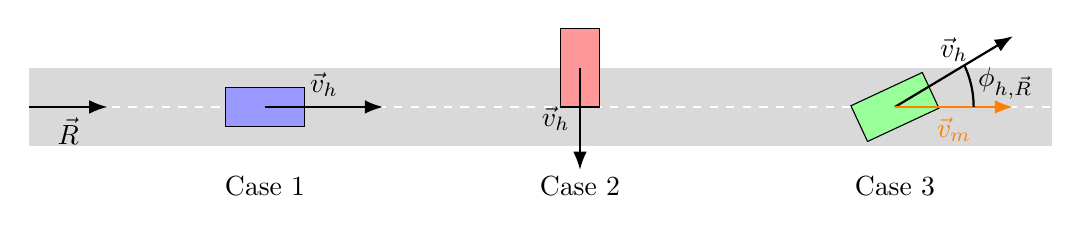
\begin{tikzpicture}

            % Draw the road as a gray rectangle
            \fill[gray!30] (-7,-0.5) rectangle (6,0.5);

            % Draw the center line of the road
            \draw[dashed, white, thick] (-7,0) -- (6,0);

            % Case 1: Vehicle driving on the road (aligned)
            \node[draw, fill=blue!40, minimum width=1cm, minimum height=0.5cm] (vehicle1) at (-4, 0) {};
            \node at (-4, -1) {Case 1};
            \draw[->, thick] (-4, 0) -- (-2.5, 0) node[midway, above] {$\vec{v}_h$};

            % Case 2: Vehicle crossing the road (perpendicular)
            \node[draw, fill=red!40, minimum width=1cm, minimum height=0.5cm, rotate=90] (vehicle2) at (0, 0.5) {};
            \node at (0, -1) {Case 2};
            \draw[->, thick] (0, 0.5) -- (0, -0.8) node[midway, left] {$\vec{v}_h$};

            % Case 3: Vehicle moving at an angle to the road
            \node[draw, fill=green!40, minimum width=1cm, minimum height=0.5cm, rotate=25] (vehicle3) at (4, 0) {};
            \node at (4, -1) {Case 3};
            \draw[->, thick] (4, 0) -- (5.5, 0.9) node[midway, above] {$\vec{v}_h$};

            % Draw the projection onto the road for Case 3
            \draw[dotted, thick] (4, 0) -- (4.5, 0);
            \draw[->, thick, orange] (4, 0) -- (5.5, 0) node[midway, below] {$\vec{v}_m$};

            % Draw the angle phi for Case 3
            \draw[thick] (5, 0) arc (0:25:1.25);
            \node at (5.4, 0.3) {$\phi_{h,\vec{R}}$};

            % Draw the road vector R
            \draw[->, thick] (-7, 0) -- (-6, 0) node[midway, below] {$\vec{R}$};
        \end{tikzpicture}
        \caption{Cases of vehicles traveling on road network}
        \label{fig:vehicleTravelingCases}
    \end{figure}




\section{Road network export and sync}\label{sec:road-network-export-and-sync}



\include{chapters/Results}
\include{chapters/FutureWork}
%%%-----------------------------------------------------------------------------
\appendix                                                             % Appendix 
%%%-----------------------------------------------------------------------------



%%%-----------------------------------------------------------------------------
\backmatter                           % Back part (bibliography, glossary, etc.)
%%%-----------------------------------------------------------------------------

\MakeBibliography % References
%%%-----------------------------------------------------------------------------
% Special page for checking print size
%%%-----------------------------------------------------------------------------

\include{back/printbox}

%%%-----------------------------------------------------------------------------
\end{document}
%%%-----------------------------------------------------------------------------
